\documentclass[a4paper, 12pt]{article}
\topmargin = -1 cm
\textheight = 650 pt
%\textwidth = 16 cm
%\oddsidemargin = -0.1 cm
\usepackage{fancyhdr}
\usepackage{amsmath}
\usepackage{graphicx}
\usepackage{shortvrb}
\usepackage[T1]{fontenc}
\usepackage[latin1]{inputenc}
\usepackage{listings} 

\begin{document}
%-----------------------------------------------------------
\begin{center}
\Huge Seminario de C++98-C++0x
\end{center}


\begin{center}

\end{center}

\section{Genericidad en C++ basados en templates.Tipos de argumentos}
La genericidad es una propiedad que permite definir una clase o una funci\'on sin tener que especificar el tipo de todos o alguno de sus miembros.\\
La utilidad principal de este tipo de clases o funciones (gen\'ericas) es la de agrupar variables cuyo tipo no est\'e predeterminado. De esta forma el funcionamiento de una pila, una cola, una lista, un conjunto, un diccionario o un array es el mismo independientemente del tipo de datos que almacene (int, long, double, char, u object de una clase definida por el usuario).
Esta propiedad no es imprescindible de un lenguaje de programaci\'on orientado a objetos. En C++ la genericidad se alcanza con los templates.\\
Un template implementa el concepto de tipo parametrizado permitiendo el concepto de genericidad en el lenguaje C++.
Le dice al compilador que la definici\'on de clase o de funci\'on que le sigue manipular\'a uno o m\'as tipos de datos no especificados.
En el momento en que el c\'odigo de la clase o de la funci\'on actual es generado, los tipos deben ser especificados para que el compilador pueda sustituirlos.\\
\subsection{Tipos de argumentos}
Las plantillas de clase y funci\'on pueden tener argumentos predeterminados. Cuando una plantilla tiene un argumento predeterminado, se puede dejar sin especificar al usarlo. Por ejemplo, la plantilla std::vector tiene un argumento predeterminado para el asignador:\\
\lstset{language=C++, breaklines=true,basicstyle=\footnotesize}
\begin{lstlisting}[frame=single]
template <class T, class Allocator = allocator<T>> class vector;
\end{lstlisting}
En la mayor\'ia de los casos, la clase std::allocator predeterminada es aceptable, por lo que se usa un vector similar al siguiente:\\
\lstset{language=C++, breaklines=true,basicstyle=\footnotesize}
\begin{lstlisting}[frame=single]
vector<int> myInts;
\end{lstlisting}
Pero si es necesario, se puede especificar un asignador personalizado de la siguiente manera:\\
\lstset{language=C++, breaklines=true,basicstyle=\footnotesize}
\begin{lstlisting}[frame=single]
vector<int, MyAllocator> ints;
\end{lstlisting}
Para varios argumentos de plantilla, todos los argumentos despu\'es del primer argumento predeterminado deben tener argumentos predeterminados.
Cuando se usa una plantilla cuyos par�metros est\'an todos predeterminados, se usan corchetes angulares vac\'ios:\\
\lstset{language=C++, breaklines=true,basicstyle=\footnotesize}
\begin{lstlisting}[frame=single]
template<typename A = int, typename B = double>
class Bar
{
    //...
};
...
int main()
{
    Bar<> bar; // use all default type arguments
}
\end{lstlisting}

\section{Definici\'on de arrays en C++}
\subsection{Definici\'on}
Un arreglo es un grupo de ubicaciones de memoria consecutivas, todas ellas del mismo tipo. Para hacer referencia a una ubicaci\'on o elemento espec\'ifico en el arreglo, especificamos su nombre y el n\'umero de posici\'on del elemento espec\'ifico en el arreglo.\\

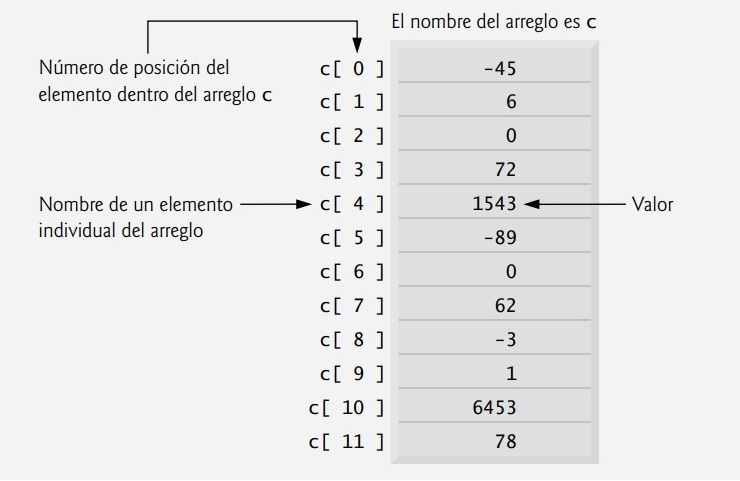
\includegraphics[scale=0.6]{img/array_1.jpg}\\[0.5cm]

En la imagen se muestra un arreglo de enteros llamado c.Este arreglo contiene 12 elementos. Para hacer referencia a cualquiera de estos elementos en un programa, se proporciona el nombre del arreglo seguido del n\'umero de posici\'on del elemento espec\'ifico entre corchetes ([]). Los nombres de los arreglos siguen las mismas 
convenciones que los dem\'as nombres de variables; es decir, deben ser identificadores.
Un sub\'indice debe ser un entero o una expresi\'on entera (usando cualquier tipo integral). Si un programa utiliza una expresi\'on como un sub\'indice, entonces el programa eval\'ua la expresi\'on para determinar el sub\'indice.\\
Ejemplo
\lstset{language=C++, breaklines=true,basicstyle=\footnotesize}
\begin{lstlisting}[frame=single]
c[ a + b ] += 2;
\end{lstlisting}

\subsection{Declaraci\'on y creaci\'on de arreglos}
Los objetos arreglo ocupan espacio en memoria. Para especificar el tipo de los elementos y el n\'umero de elementos requerido por un arreglo, use una declarac\'on de la forma: \\
tipo nombreArreglo[ tama\~noArreglo ];

El compilador reserva la cantidad apropiada de memoria. (una declaraci\'on que reserva memoria se conoce en forma m\'as apropiada como definici\'on.) El tama\~noArreglo debe ser una constante entera mayor que cero. Por ejemplo, para indicar al compilador que debe reservar 12 elementos para el arreglo c de enteros, use la siguiente declaraci\'on:\\
\lstset{language=C++, breaklines=true,basicstyle=\footnotesize}
\begin{lstlisting}[frame=single]
int c[ 12 ]; // c es un arreglo de 12 enteros
\end{lstlisting}

Se puede reservar memoria para varios arreglos con una sola declaraci\'on. La siguiente declaraci\'on reserva 100 elementos para el arreglo b de enteros y 27 elementos para el arreglo x de enteros.\\
\lstset{language=C++, breaklines=true,basicstyle=\footnotesize}
\begin{lstlisting}[frame=single]
int b[ 100 ]; // b es un arreglo de 100 enteros\\
x[ 27 ]; // x es un arreglo de 27 enteros\\
\end{lstlisting}
	
\subsection{Inicializaci\'on}
Los elementos de un arreglo tambi\'en se pueden inicializar en la declaraci\'on del arreglo, para lo cual colocamos despu\'es 
del nombre del arreglo un signo igual y una lista entre llaves, separada por comas, de inicializadores.
Si hay menos inicializadores que elementos en el arreglo, el resto de los elementos del arreglo se inicializan con cero. \\
Por ejemplo:\\
\lstset{language=C++, breaklines=true,basicstyle=\footnotesize}
\begin{lstlisting}[frame=single]
int n[ 10 ] = {}; // inicializa los elementos del arreglo n con 0
\end{lstlisting}

Si el tama\~no del arreglo se omite en una declaraci\'on con una lista inicializadora, el compilador determina el n\'umero 
de elementos en el arreglo mediante un conteo del n\'umero de elementos en la lista inicializadora. Por ejemplo\\
\lstset{language=C++, breaklines=true,basicstyle=\footnotesize}
\begin{lstlisting}[frame=single]
int n[] = { 1, 2, 3, 4, 5 };\\
\end{lstlisting}
crea un arreglo de cinco elementos.\\
Si se especifican el tama\~no del arreglo y una lista inicializadora en la declaraci\'on de un arreglo, el n\'umero de inicializadores debe ser menor o igual que el tama\~no del arreglo. La declaraci\'on del arreglo\\
\lstset{language=C++, breaklines=true,basicstyle=\footnotesize}
\begin{lstlisting}[frame=single]
int n[ 5 ] = { 32, 27, 64, 18, 95, 14 };\\
\end{lstlisting}
produce un error de compilaci\'on, ya que hay 6 inicializadores y s\'olo 5 elementos en el arreglo.\\
\section{Distintos tipos de constructores en C++(defecto y copia)}
Un constructor es una funci\'on que es autom\'aticamente llamada cuando se necesita inicializar variables o asignar memoria din\'amica durante el proceso de creaci\'on de un objeto y as\'i evitar que se obtengan valores inesperados.Los constructores no tiene asignado ning\'un tipo de retorno, ni siquiera void y deben tener el mismo nombre de la clase.Los constructores se pueden sobrecargar, o sea definir varios constructores (con el mismo nombre) pero deben diferir al menos una vez en el tipo o la cantidad de par\'ametros.

\subsection{�Qu\'e hace cada uno de ellos?}
\begin{itemize}
\item CONSTRUCTOR POR DEFECTO Y CONSTRUCTOR CON PAR\'AMETROS CON VALOR POR DEFECTO\\
Se llama constructor por defecto a un constructor que no necesita que se le pasen par\'ametros o argumentos para inicializar las variables miembro de la clase. Un constructor por defecto es pues un constructor que no tiene argumentos o que, si los tiene, todos sus argumentos tienen asignados un valor por defecto en la declaraci\'on del constructor. En cualquier caso, puede ser llamado sin tenerle que pasar ning\'un argumento.
\item CONSTRUCTOR DE OFICIO\\
\begin{itemize}
\item Es un constructor generado autom\'aticamente por C++ que no recibe par\'ametros.
\item No se crea en el caso que se haya definido otro constructor.
\item Inicia todas las variables miembro a 0. Aunque esto no es razonable en todos los contextos.
\end{itemize}
\item CONSTRUCTOR DE COPIA\\
En C++ se obliga a inicializar las variables miembro de una clase llamando a un constructor, cada vez que se crea un objeto de dicha clase. Se ha comentado tambi\'en que el constructor puede recibir como par\'ametros los valores que tiene que asignar a las variables miembro, o puede asignar valores por defecto.Por definici\'on, el
constructor de copia tiene un \'unico argumento que es una referencia constante a un objeto de la clase. Su declaraci\'on ser\'ia:
\lstset{language=C++, breaklines=true,basicstyle=\footnotesize}
\begin{lstlisting}[frame=single]
C_Cuenta(const C_Cuenta&);
\end{lstlisting}
El constructor de copia de oficio se limita a realizar una copia bit a bit de las variables miembro del objeto original al objeto copia. Hay casos en lo que la copia bit a bit no
da los resultados esperados. En este caso el programador debe preparar su propio constructor de copia e incluirlo en la clase como un constructor sobrecargado m\'as.Este surge si no se crea un constructor de copia.\\
\item CONSTRUCTOR CON ARGUMENTOS\\
\begin{itemize}
\item Representa un constructor que recibe uno o varios argumentos como par\'ametros.
\item Debe llamarse pas\'andole al menos 1 argumento. En este caso todos los demas ser\'an argumentos que tengan algun valor por defecto.
\end{itemize}
\end{itemize}
\subsection{�Cu\'ando se llaman?}
Los constructores se llaman para crear una instancia del objeto en cuesti\'on.\\
Se pueden llamar utilizando el operador new que reserva memoria din\'amicamente y retorna un puntero al inicio del bloque de la misma.

\begin{itemize}
\item CONSTRUCTOR POR DEFECTO Y CONSTRUCTOR CON PAR�METROS CON VALOR POR DEFECTO
El constructor por defecto es necesario si se quiere hacer una declaraci\'on en la forma:
\lstset{language=C++, breaklines=true,basicstyle=\footnotesize}
\begin{lstlisting}[frame=single]
C_Cuenta c1;
\end{lstlisting}
y tambi\'en cuando se quiere crear un vector de objetos, por ejemplo en la forma:
\lstset{language=C++, breaklines=true,basicstyle=\footnotesize}
\begin{lstlisting}[frame=single]
C_Cuenta cuentas[100];
\end{lstlisting}
ya que en este caso se crean e inicializan m\'ultiples objetos sin poderles pasar argumentos
personalizados o propios para cada uno de ellos.

El constructor puede tener definidos unos valores por defecto para los par\'ametros, que se asignen a las variables miembro de la clase. Esto es especialmente \'util en el caso de que una variable miembro repita su valor para todos o casi todos los objetos de esa clase que se creen. Consid\'erese el ejemplo siguiente:
\lstset{language=C++, breaklines=true,basicstyle=\footnotesize}
\begin{lstlisting}[frame=single]
class C_Cuenta {
// Variables miembro
private:
double Saldo;          // Saldo Actual de la cuenta
double Interes;       // Inter�s aplicado

public:
C_Cuenta(double unSaldo=0.0, double unInteres=0.0)  // Constructor
{
     SetSaldo(unSaldo);
     SetInteres(unInteres);
}
};
\end{lstlisting}
\item CONSTRUCTOR DE COPIA
El constructor de copia se llama cuando se necesita crear un objeto nuevo a partir de otro objeto.\\
Surge la necesidad de escribir un constructor de copia distinto del que proporciona el compilador en casos en los que la copia bit a bit no resulta.

Fig:\\
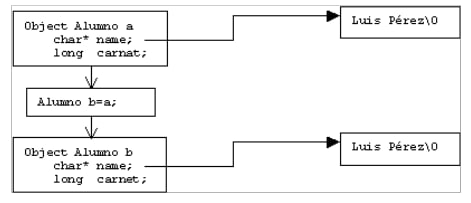
\includegraphics[scale=0.6]{img/photo_2022-10-16_12-38-50.jpg}\\[0.5cm]\\

La situaci\'on mostrada en la figura 2 puede tener consecuencias no deseadas. Por ejemplo, si
se quiere cambiar el nombre del Alumno a, lo primero que se hace es liberar la memoria a la que apunta a.nombre, reservar memoria para el nuevo nombre haciendo que a.nombre apunte al
comienzo de dicha memoria, y almacenar all\'i el nuevo nombre de a. Como el objeto b no se ha tocado, su variable miembro b.nombre se ha quedado apuntado a una posici\'on de memoria que ha sido liberada en el proceso de cambio de nombre de a.La consecuencia es que b ha perdido informaci\'on y los m\'as probable es que el programa falle.\\
Se llega a una situaci\'on parecida cuando se destruye uno de los dos objetos a o b. Al destruir uno de los objetos se libera la memoria que comparten, con el consiguiente perjuicio para el objeto que queda, puesto que su puntero contiene la direcci\'on de una zona de memoria liberada, disponible para almacenar otra informaci\'on.\\

Fig:\\
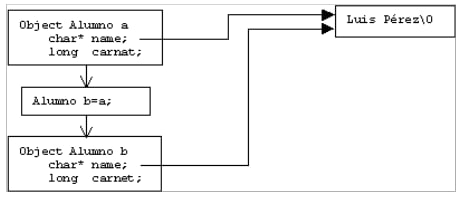
\includegraphics[scale=0.6]{img/photo_2022-10-16_12-38-33.jpg}\\[0.5cm]

La figura  muestra la situaci\'on a la que se llega con un constructor de copia
correctamente programado por el usuario. En este caso, el constructor no copia bit a bit la direcci\'on contenida en a.nombre, sino que reserva memoria, copia a esa memoria el contenido apuntado por a.nombre, y guarda en b.nombre la direcci\'on de esa nueva memoria reservada. Ninguno de los problemas anteriores sucede ahora.
\end{itemize}
\subsection{Inicializaci\'on de campos}
Como sabemos C++ no permite crear objetos sin dar un valor inicial apropiado a todas sus
variables miembro. Esto se hace por medio de unas funciones llamadas constructores, que se
llaman autom\'aticamente siempre que se crea un objeto de una clase.\\
La idea del constructor es inicializar variables, y una sentencia de
asignaci\'on no es la \'unica ni la mejor forma de inicializar una variable. C++ permite inicializar variables miembro fuera del cuerpo del constructor, de la siguiente forma:\\
\lstset{language=C++, breaklines=true,basicstyle=\footnotesize}
\begin{lstlisting}[frame=single]
C_Cuenta::C_Cuenta(double unSaldo, double unInteres) :
                  Saldo(unSaldo), Interes(unInteres)   // inicializadores
{// En este caso el cuerpo del constructor est� vac�o }
\end{lstlisting}
donde se ve que los inicializadores se introducen, tras el car\'acter dos puntos (:), separados por comas, justo antes de abrir las llaves del cuerpo del constructor. Constan del nombre de la variable miembro seguido, entre par\'entesis, del argumento que le da valor. Los inicializadores son m\'as eficientes que las sentencias de asignaci\'on, y adem\'as permiten definir variables miembro const, que pueden ser inicializadas pero no asignadas.


\subsection{�C\'omo funciona el paso de par\'ametros cuando se llama a una funci\'on?}
Los par\'ametros se comportan como cualquier otra variable dentro de la funci\'on. 
El paso de par\'ametros en C++ se puede hacer de dos formas:
\begin{itemize}
\item Paso de par\'ametros por valor.
\item Paso de par\'ametros por referencia.
\end{itemize}

\subsection{�Cu\'ando se deben utilizar par\'ametros por valor, por puntero o por referencia?}
\begin{itemize}
\item Paso de par\'ametros por valor.\\
Pasar par\'ametros por valor significa que a la funci\'on se le pasa una copia del valor que contiene el par\'ametro actual.
Los valores de los par\'ametros de la llamada se copian en los par\'ametros de la cabecera de la funci\'on. La funci\'on trabaja con una copia de los valores por lo que cualquier modificaci\'on en estos valores no afecta al valor de las variables utilizadas en la llamada.
Aunque los par\'ametros actuales (los que aparecen en la llamada a la funci\'on) y los par\'ametros formales (los que aparecen en la cabecera de la funci\'on) tengan el mismo nombre son variables distintas que ocupan posiciones distintas de memoria.
Por defecto, todos los argumentos salvo los arrays se pasan por valor. \\
\item Paso de par\'ametros por referencia.\\
Hay dos formas de pasar los par\'ametros por referencia:
\begin{itemize}
\item Paso de par\'ametros por referencia basado en punteros
\item Paso de par\'ametros por referencia usando referencias al estilo C++.
\end{itemize}
\item Paso de par�metros por referencia basado en punteros\\
Cuando se pasan par\'ametros por referencia, se le env\'ia a la funci\'on la direcci\'on de memoria del par\'ametro actual y no su valor. La funci\'on realmente est\'a trabajando con el dato original y cualquier modificaci\'on del valor que se realice dentro de la funci\'on se estar\'a realizando con el par\'ametro actual.
Para recibir la direcci\'on del par\'ametro actual, el par\'ametro formal debe ser un puntero.\\
Ejemplo 1:\\
Programa c++ que lee dos n\'umeros por teclado y los env\'ia a una funci\'on para que intercambie sus valores.\\
 \lstset{language=C++, breaklines=true,basicstyle=\footnotesize}
 \begin{lstlisting}[frame=single]
#include <iostream>
using namespace std;
void intercambio(int *, int *);
int main( )
{
    int a, b;
    cout << "Introduce primer numero: ";
    cin >> a;
    cout << "Introduce segundo numero: ";
    cin >> b;
    cout << endl;
    cout << "valor de a: " << a << " valor de b: " << b << endl;
    intercambio(&a, &b); 
    cout << endl << "Despues del intercambio: " << endl << endl;
    cout << "valor de a: " << a << " valor de b: " << b << endl;
    system("pause");
}
void intercambio(int *x, int *y)
{
    int z;                      
    z = *x;
    *x = *y;
    *y = z;
}
 \end{lstlisting}
En la llamada, a la funci\'on se le env\'ia la direcci\'on de los par\'ametros. El operador que obtiene la direcci\'on de una variable es \&.
\lstset{language=C++, breaklines=true,basicstyle=\footnotesize}
\begin{lstlisting}[frame=single]
intercambio(&a, &b); 
\end{lstlisting}
En la cabecera de la funci\'on, los par\'ametros formales que reciben las direcciones deben ser punteros. Esto se indica mediante el operador *
\lstset{language=C++, breaklines=true,basicstyle=\footnotesize}
\begin{lstlisting}[frame=single]
 void intercambio(int *x, int *y)
\end{lstlisting}
Los punteros x e y reciben las direcciones de memoria de las variables a y b. Al modificar el contenido de las direcciones x e y, indirectamente estamos modificando los valores a y b. Por tanto, pasar par\'ametros por referencia a una funci\'on es hacer que la funci\'on acceda indirectamente a las variables pasadas. \\
\item Paso de par�metros por referencia usando referencias al estilo C++
Una referencia es un nombre alternativo (un alias, un sin\'onimo) para un objeto. Una referencia no es una copia de la variable referenciada, sino que es la misma variable con un nombre diferente.
Utilizando referencias, las funciones trabajan con la misma variable utilizada en la llamada. Si se modifican los valores en la funci\'on, realmente se est\'an modificando los valores de la variable original.\\
Ejemplo:\\
El primer ejemplo del punto anterior utilizando referencias lo podemos escribir as\'i:\\
\lstset{language=C++, breaklines=true,basicstyle=\footnotesize}
\begin{lstlisting}[frame=single]
#include <iostream>
using namespace std;
void intercambio(int &, int &);
int main( )
{   int a, b;
    cout << "Introduce primer numero: ";
    cin >> a;
    cout << "Introduce segundo numero: ";
    cin >> b;
    cout << endl;
    cout << "valor de a: " << a << " valor de b: " << b << endl;
    intercambio(a, b); 
    cout << endl << "Despues del intercambio: " << endl << endl;
    cout << "valor de a: " << a << " valor de b: " << b << endl;
    system("pause");
}
void intercambio(int &x, int &y)
{
    int z;                      
    z = x;
    x = y;
    y = z;
}
\end{lstlisting}
En la declaraci\'on de la funci\'on y en la definici\'on se coloca el operador referencia a \& en aquellos par\'ametros formales que son referencias de los par\'ametros actuales:\\
\lstset{language=C++, breaklines=true,basicstyle=\footnotesize}
\begin{lstlisting}[frame=single]
void intercambio(int &, int &);   //declaraci�n de la funci�n
void intercambio(int &x, int &y)  //definici�n de la funci�n
\end{lstlisting}
Cuando se llama a la funci\'on:\\
\lstset{language=C++, breaklines=true,basicstyle=\footnotesize}
\begin{lstlisting}[frame=single]
intercambio(a, b); 
\end{lstlisting}
se crean dos referencias (x e y) a las variables a y b de la llamada. Lo que se haga dentro de la funci\'on con x e y se est\'a haciendo realmente con a y b.\\
\end{itemize}

\subsection{Constructores con un solo argumento}
Converting constructor o Constructores con un solo argumento:\\
Representa un constructor que recibe un solo argumento como par\'ametro
Un constructor declarado sin el especificador de funci\'on explicit que se puede llamar con un solo par\'ametro especifica una conversi\'on del tipo de su primer par\'ametro al tipo de su clase. Tal constructor se llama constructor de conversi\'on.\\
Ejemplo:
\lstset{language=C++, breaklines=true,basicstyle=\footnotesize}
\begin{lstlisting}[frame=single]
class MyClass
{
  public:
     int a, b;
     MyClass( int i ) {}
     MyClass( const char* n, int k = 0 ) {}
     MyClass( MyClass& obj ) {}
}
\end{lstlisting}
Para ser un constructor de conversi\'on, el constructor debe tener un solo argumento (en el segundo, el segundo argumento tiene un valor predeterminado) y ser declarado sin la palabra clave explicit.\\

\subsection{Constructores explicit}
Fuerza al programador a que se haga un cast explicito sobre el objeto que recibe el constructor de un solo argumento de la clase al tipo del objeto que se esta creando, evitando as\'i que se efect�en operaciones de cast impl\'icitas.\\
Ejemplo:\\
\lstset{language=C++, breaklines=true,basicstyle=\footnotesize}
\begin{lstlisting}[frame=single]
class MyClass
{
  public:
     int a, b;
     explicit MyClass( int i ) {}
}
\end{lstlisting}
Entonces, el compilador no aceptar\'ia\\
\lstset{language=C++, breaklines=true,basicstyle=\footnotesize}
\begin{lstlisting}[frame=single]
 	int main()
    {
        MyClass M = 1 ;
    }
\end{lstlisting}
Ya que esto es conversi\'on impl\'icita. En su lugar, tienen que escribir\\
\lstset{language=C++, breaklines=true,basicstyle=\footnotesize}
\begin{lstlisting}[frame=single]
 	int main()
    {
        MyClass M(1) ;
        MyClass M = MyClass(1) ;
        MyClass* M = new MyClass(1) ;
        MyClass M = (MyClass)1;
        MyClass M = static_cast<MyClass>(1);
    }
\end{lstlisting}
explicit la palabra clave siempre se usa para evitar la conversi\'on impl\'icita de un constructor y se aplica al constructor en una declaraci\'on de clase.

\section{Funciones inline y const}
Funcion inline:\\
En la mayor\'ia de los casos la programaci\'on orientada a objetos obliga a utilizar funciones para poder acceder a las variables miembro de una clase. Por esta raz\'on un programa orientado a objetos contiene muchas llamadas a funciones. Por otra parte, muchas de las funciones que se utilizan contienen s\'olo unas pocas sentencias o incluso una sola, por ejemplo las funciones de lectura y asignaci\'on de valores de una variable.\\
Cada llamada y retorno de una funci\'on tiene un cierto costo computacional, porque es
necesario reservar una zona de memoria para los argumentos de las funciones llamadas, que a
veces, adem\'as tienen que ser copiados. En la mayor\'ia de los casos el tiempo empleado en la transmisi\'on de datos es despreciable frente al empleado en los c\'alculos. En el caso de que la funci\'on sea muy sencilla, sin embargo, no se puede despreciar ese tiempo y el uso frecuente de funciones muy sencillas y breves se revela muy poco eficiente.\\
La expansi\'on inline ofrece la soluci\'on a este problema sustituyendo en el programa la
llamada a la funci\'on por el c\'odigo de la misma, modificado para simular el paso de argumentos y valor de retorno. Las funciones inline eliminan la necesidad de utilizar las macros de C.\\
La ventajas de las funciones inline vienen dadas porque su utilizaci\'on puede suponer una
reducci\'on del tiempo de ejecuci\'on de un programa. El inconveniente de usar funciones inline es que la introducci\'on de una copia del c\'odigo en cada llamada a una funci\'on puede hacer que el tama\~no del programa aumente considerablemente. En definitiva, el uso de este tipo de funciones est\'a recomendado en el caso de que sean funciones muy sencillas cuyo tiempo de llamada es comparable al tiempo de c\'alculo. Por el contrario, en el caso de funciones m\'as grandes, la mejora en el tiempo de ejecuci\'on es despreciable y el tama\~no del programa puede crecer innecesariamente.\\

Funcion const:\\
En C++ el especificador const se puede utilizar con variables y con punteros. Las variables
definidas como const no son lo mismo que las constantes simb\'olicas, aunque evidentemente hay una cierta similitud en las \'areas de aplicaci\'on. Si una variable se define como const se tiene la garant\'ia de que su valor no va a cambiar durante toda la ejecuci\'on del programa. Si en alguna sentencia del programa se intenta variar el valor de una variable definida como const, el compilador produce un mensaje de error. Esta precauci\'on permite detectar errores durante la compilaci\'on del programa, lo cual siempre es m\'as sencillo que detectarlos en tiempo de ejecuci\'on.\\
Las variables de este tipo pueden ser inicializadas pero no pueden estar a la izquierda de una sentencia de asignaci\'on.\\
Las variables declaradas como const tienen importantes diferencias con las constantes
simb\'olicas definidas con la directiva define del preprocesador. Aunque ambas representan valores que no se puede modificar, las variables const est\'an sometidas a las mismas reglas de visibilidad y duraci\'on que las dem\'as variables del lenguaje.\\
Las variables const de C++ pueden ser utilizadas para definir el tama\~no de un vector en la
declaraci\'on de \'este, cosa que no est\'a permitida en C.\\
Es muy frecuente que las funciones a las que por motivos de eficiencia (para no tener que
sacar copias de los mismos) se les pasan los argumentos por referencia, \'estos ser\'an declarados como const en la definici\'on y en el prototipo de la funci\'on, con objeto de hacer imposible una modificaci\'on accidental de dichos datos. Esto sucede por ejemplo con las funciones de manejo de cadenas de caracteres. El prototipo de la funci\'on strcpy() puede ser como sigue:\\
\lstset{language=C++, breaklines=true,basicstyle=\footnotesize}
\begin{lstlisting}[frame=single]
char *strcpy(char *s1, const char *s2);
\end{lstlisting}
\subsection{Implementaci\'on de las funciones inline}
C++ permite 2 maneras distintas de implementar funciones inline\\
En el caso de los punteros hay que distinguir entre dos formas de aplicar el cualificador const:
\begin{enumerate}
\item La primera de ellas consiste en colocar la palabra inline precediendo a la definici\'on de la funci\'on:\\
\lstset{language=C++, breaklines=true,basicstyle=\footnotesize}
\begin{lstlisting}[frame=single]
inline double funcion (double uno)
{return uno;}
\end{lstlisting}
Es importante saber que esta indicaci\'on puede ser ignorada por el compilador en el caso de que la funci\'on en cuesti\'on sea tan larga o tan complicada que su expansi\'on inline resulte desaconsejable. De todos modos, el que se produzca o no la expansi\'on de la funci\'on no hace variar nada la definici\'on de la misma.\\
La definici\'on de las funciones inline debe hacerse en los ficheros de encabezamiento
(extensi\'on *.h), y no en los ficheros fuente (extensi\'on *.cpp). Cada vez que se utiliza una funci\'on inline su llamada es sustituida por el c\'odigo de la misma, por lo que o\'iste debe ser accesible para cualquier fichero fuente, y eso se consigue incluyendola en el fichero header.\\
\item El segundo m\'etodo de declaraci\'on de funciones inline consiste en colocar la definici\'on completa de la misma en la declaraci�n de la funci\'on:\\
\lstset{language=C++, breaklines=true,basicstyle=\footnotesize}
\begin{lstlisting}[frame=single]
class una {
 double tal;
 public:
 double Expandida( )
 { return tal;}
};
\end{lstlisting}
En el caso de que se incluya la definici\'on de una funci\'on inline en una clase, esta misma definici\'on sirve tambi\'en como declaraci\'on. Estas definiciones pueden incluir argumentos por defecto.
Tal como se han definido las funciones, incluyendo su definici\'on en la declaraci\'on, estas funciones ya eran inline. En el siguiente ejemplo se a\~nade la palabra inline, aunque no es necesaria, para subrayar esta caracter\'istica de las funciones:
\lstset{language=C++, breaklines=true,basicstyle=\footnotesize}
\begin{lstlisting}[frame=single]
class C_Cuenta {
 // Variables miembro
private: // La palabra private no es necesaria
char *Nombre; // Nombre de la persona
double Saldo; 
double Interes; // Inter�s aplicado
public:
// M�todos
inline char *GetNombre() // La palabra inline no es necesaria
{ return Nombre; }
inline double GetSaldo()
 { return Saldo; }
 inline double GetInteres()
 { return Interes; }
 inline void SetSaldo(double unSaldo)
 { Saldo = unSaldo; }
 inline void SetInteres(double unInteres)
 { Interes = unInteres; }
 void Ingreso(double unaCantidad)
 { SetSaldo( GetSaldo() + unaCantidad ); }
\end{lstlisting}
\end{enumerate}
\subsection{Diferencia entre const T x; T const x; y const T const x;}
No existe diferencia entre const T x y T const x, es decir el calificador const se aplica a lo que est\'a inmediatamente a su izquierda, si no hay nada a su izquierda, se aplica a lo que esta inmediatamente a su derecha. Por tanto para estar en armon\'ia con la regla 'Derecha Izquierda' se recomienda que es mejor escribir T const x.\\
Sin embargo cambia cuando son punteros es decir const T *x y T* const x, son diferentes, al igual que const T *const x.\\
\subsection{Funci\'on const para punteros}
Existen dos formas de aplicar el cualificador const:
\begin{enumerate}
\item un puntero variable apuntando a una variable constante 
\item un puntero constante apuntando a una variable cualquiera
\end{enumerate}
Un puntero a una variable const no puede modificar el valor de esa variable (si se intentase el compilador lo detectar\'ia e imprimir\'ia un mensaje de error), pero ese puntero no tiene por qu\'e apuntar siempre a la misma variable.
En el caso de un puntero const, \'este apunta siempre a la misma direcci\'on de memoria pero el valor de la variable almacenada en esa direcci\'on puede cambiar sin ninguna dificultad.
Un puntero a variable const se declara anteponiendo la palabra const:
\lstset{language=C++, breaklines=true,basicstyle=\footnotesize}
\begin{lstlisting}[frame=single]
const char *nombre1 "Ram�n" // no se puede modificar el valor de la variable
\end{lstlisting}
Por otra parte, un puntero const a variable cualquiera se declara interponiendo la palabra
const entre el tipo y el nombre de la variable:
\begin{lstlisting}[frame=single]
char* const nombre2 "Ram�n" // no se puede modificar la direcci�n a la que apunta el puntero, pero s� el valor.
\end{lstlisting}
En ANSI C una variable declarada como const puede ser modificada a trav\'es de un puntero a
dicha variable. Por ejemplo, el siguiente programa compila y produce una salida i=3 con el
compilador de C, pero da un mensaje de error con el compilador de C++:\\

\lstset{language=C++, breaklines=true,basicstyle=\footnotesize}
\begin{lstlisting}[frame=single]
#include <stdio.h>
void main(void)
{
 const int i = 2;
 int *p;
 p = &i;
 *p = 3;
 printf("i=%d", i);
 }
\end{lstlisting}
\section{Redefinici\'on de operadores [] y +.Tipos de traspasos en C++}
Los operadores de C++, al igual que las funciones, pueden ser sobrecargados (overloaded). Este es uno de los aspectos m\'as caracter\'isticos de este lenguaje. La sobrecarga de operadores quiere decir que se pueden redefinir algunos de los operadores existentes en C++ para que act\'uen de una determinada manera, definida por el programador, con los objetos de una clase determinada.\\
Los programadores pueden usar operadores con tipos definidos por el usuario tambi\'en. Aunque C++ no permite crear nuevos operadores, s\'i permite sobrecargar la mayor\'ia de los operadores existentes para que, cuando \'estos se utilicen con objetos, tengan un significado apropiado. Es una poderosa herramienta.\\
Para sobrecargar un operador, se escribe la definici\'on de una funci\'on miembro no static o la definici\'on de una funci\'on global como se hace normalmente, excepto que el nombre de la funci\'on se convierte ahora en la palabra clave operator, seguida del s\'imbolo del operador que se va a sobrecargar.\\
En el caso de la funcion operador + se utilizar\'ia para sobrecargar el operador de suma.
Cuando los operadores se sobrecargan como funciones miembro, deben ser no static, debido a que se deben llamar en un objeto de la clase y deben operar en ese objeto.\\
El significado de la forma en que trabaja un operador con objetos de tipos fundamentales no se puede modificar mediante la sobrecarga de operadores. Por ejemplo, no podemos modificar el significado de la forma en como + suma dos enteros. La sobrecarga de operadores funciona s\'olo con objetos de los tipos definidos por el usuario, o con una mezcla de un objeto de un tipo definido por el usuario y un objeto de un tipo fundamental.\\
Al sobrecargar [] operador para indexar o cualquiera de los operadores de asignaci\'on,la funci\'on de sobrecarga de operadores debe declararse como una clase miembro. Para los otros operadores, las funciones de sobrecarga de operadores pueden ser clases miembro o funciones globales.\\
Cuando una funci\'on de operador se implementa como funci\'on miembro, el operando de m\'as a la izquierda (o el �nico) debe ser un objeto (o una referencia a un objeto) de la clase del operador. Si el operando izquierdo debe ser un objeto de una clase distinta o de un tipo fundamental, esta funci\'on de operador se debe implementar como una funci\'on global.\\
Ejemplo\\
\newpage
\lstset{language=C++, breaklines=true,basicstyle=\footnotesize}
\begin{lstlisting}[frame=single]
// operador de sub\'indice sobrecargado para objetos Array no const;
// la devoluci\'on de una referencia crea un lvalue modificable
int &Array::operator[ ]( int subindice )
{
// comprueba error de sub�ndice fuera de rango
	if ( subindice < 0 || subindice >= tamano )
 	 {
	  cerr << "\nError: subindice " << subindice 
	  << "fuera_de_rango" << endl;
	  exit( 1 ); // termina el programa; subindice fuera de rango
	  } // fin de if
	  
	  return ptr[ subindice ]; // devuelve una referencia
  } // fin de la funci�n operator[]
  
  
  int main()
  {
  	Array enteros1[7]={1,2,3,4,5,6,7}; // objeto Array de 7 elementos
    Array enteros2; // objeto Array de 10 elementos de manera predeterminada
    
    // usa el operador de sub�ndice sobrecargado para crear rvalue
    cout << "\nenteros1[5] es " << enteros1[ 5 ];
    
    // usa el operador de sub�ndice sobrecargado para crear lvalue
    cout << "\n\nAsignando 1000 a enteros1[5]" << endl;
    enteros1[5]=1000;
    
    // trata de usar un sub�ndice fuera de rango
    cout << "\nTrata de asignar 1000 a enteros1[15]" << endl;
    enteros1[ 15 ] = 1000; // ERROR: fuera de rango
    return 0;
  }
\end{lstlisting}
Se utiliza el operador de sub\'indice sobrecargado para hacer referencia a enteros1[ 5 ]: un elemento de enteros1 dentro del rango. Este nombre con sub�ndice se utiliza como rvalue para imprimir el valor asignado a enteros1[ 5 ]. Mas abajo se utiliza enteros1[ 5 ] como un lvalue modificable del lado izquierdo de una instrucci�n de asignaci�n para asignar un nuevo valor, 1000, al elemento 5 de enteros1.\\
En la l�nea se trata de asignar el valor 1000 a enteros1[ 15 ]; un elemento fuera de rango. En este ejemplo, operator[ ] determina que el sub\'indice est\'a fuera de rango, imprime un mensaje y termina el programa. Observe que resaltamos la ls \'ultimas lineas del programa para enfatizar que es un error acceder a un elemento que est\'a fuera de rango. \'Este es 
un error l\'ogico en tiempo de ejecuci\'on.\\
Se puede observar que el operador de sub\'indice de arreglo [] no est\'a restringido para usarlo s\'olo con arreglos; por ejemplo, tambi\'en se puede utilizar para seleccionar elementos de otros tipos de clases contenedoras, como listas enlazadas, cadenas y diccionarios. Adem\'as, cuando se definen las funciones operator[ ], los sub\'indices ya no tienen que ser enteros; tambi\'en se pueden usar caracteres, cadenas, n\'umeros de punto flotante o incluso objetos de clases definidas por el usuario.\\

\section{Especializaci\'on de los templates}
En algunos casos, no es posible o deseable que una plantilla defina exactamente el mismo c\'odigo para cualquier tipo. Por ejemplo, es posible que se desee definir una ruta de acceso de c�digo que se va a ejecutar solo si el argumento de tipo es un puntero, o un tipo derivado de una clase base determinada. En tales casos, se puede definir una especializaci\'on de la plantilla para ese tipo determinado. Cuando un usuario crea una instancia de la plantilla con ese tipo, el compilador usa la especializaci\'on para generar la clase y para todos los dem\'as tipos, el compilador elige la plantilla m\'as general. Las especializaciones en las que todos los par\'ametros est�n especializados son especializaciones completas. Si solo algunos de los par\'ametros est\'an especializados, se denomina especializaci\'on parcial.\\
\lstset{language=C++, breaklines=true,basicstyle=\footnotesize}
\begin{lstlisting}[frame=single]
template <typename K, typename V>
class MyMap{/*...*/};

// partial specialization for string keys
template<typename V>
class MyMap<string, V> {/*...*/};
...
MyMap<int, MyClass> classes; // uses original template
MyMap<string, MyClass> classes2; // uses the partial specialization
\end{lstlisting}
Una plantilla puede tener cualquier n\'umero de especializaciones siempre que cada par\'ametro de tipo especializado sea \'unico. Solo las plantillas de clase pueden estar parcialmente especializadas. Todas las especializaciones completas y parciales de una plantilla deben declararse en el mismo espacio de nombres que la plantilla original.\\

La generalidad es una propiedad que permite definir una clase o una funci\'on sin tener que
especificar el tipo de todos o alguno de sus miembros.La utilidad principal de este tipo de clases o funciones es la de agrupar variables cuyo tipo no est\'e predeterminado. As\'i el funcionamiento de una pila, una cola, una lista, un conjunto, un diccionario o un array es el mismo independientemente del tipo de datos que almacene (int, long, double, char, u objetos de una clase definida por el usuario). En definitiva estas clases se definen
independientemente del tipo de variables que vayan a contener y es el usuario de la clase el que debe indicar ese tipo en el momento de crear un objeto de esa clase.\\
\subsection{Templates de funciones}
Si se quiere crear una funci\'on que devolviese el m\'inimo entre dos valores independientemente de su tipo (se supone que ambos tienen el mismo tipo). Se podr\'ia pensar en definir la funci\'on tantas veces como tipos de datos se puedan presentar (int, long, float, double, etc.). Aunque esto es posible, \'este es un caso ideal para aplicar plantillas de funciones. Esto se puede hacer de la siguiente manera:
\lstset{language=C++, breaklines=true,basicstyle=\footnotesize}
\begin{lstlisting}[frame=single]
// Declaraci�n de la plantilla de funci�n
template <class T> T minimo( T a, T b);
\end{lstlisting}
En ese caso con <classT> se est\'a indicando que se trata de una plantilla cuyo par\'ametro va a ser el tipo T y que tanto el valor de retorno como cada uno de los dos argumentos va a ser de este tipo de dato T. En la definici\'on y declaraci\'on de la plantilla puede ser que se necesite utilizar mas de un tipo de dato e incluido alg\'un otro par\'ametro constante que pueda ser utilizado en las declaraciones. Por ejemplo, si hubiera que pasar dos tipos a la plantilla, se podr\'ia escribir:
\lstset{language=C++, breaklines=true,basicstyle=\footnotesize}
\begin{lstlisting}[frame=single]
// Declaraci�n de la plantilla de funci�n con dos tipos de datos
template <class T1, class T2> void combinar(T1 a, T2 b);
\end{lstlisting}
Podr\'ia darse el caso tambi\'en de que alguno de los argumentos o el valor de retorno fuese de un tipo de dato constante y conocido. En ese caso se indicar\'ia expl\'icitamente como en una funci\'on convencional.\\
\lstset{language=C++, breaklines=true,basicstyle=\footnotesize}
\begin{lstlisting}[frame=single]
// Definici�n de la plantilla de funci�n
template <class T> T minimo(T a, T b)
{
 if(a <= b)
 return a;
 else
 return b;
}
\end{lstlisting}
Ejemplo donde se utiliza la plantilla de funci\'on reci\'en definida
\lstset{language=C++, breaklines=true,basicstyle=\footnotesize}
\begin{lstlisting}[frame=single]
#include <iostream.h>
template <class T> T minimo(T a, T b);
void main(void)
{
 int euno=1;
 int edos=5;
 cout << minimo(euno, edos) << endl;
 long luno=1;
 long ldos=5;
 cout << minimo(luno, ldos) << endl;
 char cuno='a';
 char cdos='d';
 cout << minimo(cuno, cdos) << endl;
 double duno=1.8;
 double ddos=1.9;
 cout << minimo(duno, ddos) << endl;
}
\end{lstlisting}
La ejecuci\'on del programa anterior demuestra que el tipo de los argumentos y el valor de
retorno de la funci\'on minimo() se particularizan en cada caso a los de la llamada.\\
De forma general como se puede apreciar un template de funcion ser\'ia:
\lstset{language=C++, breaklines=true,basicstyle=\footnotesize}
\begin{lstlisting}[frame=single]
template <class identifier> function_declaration;
\end{lstlisting}
\subsection{Templates de clases}
De una manera semejante a como se hace para las funciones se puede generalizar para el caso de las clases por medio de plantillas de clases.\\
\lstset{language=C++, breaklines=true,basicstyle=\footnotesize}
\begin{lstlisting}[frame=single]
template <class identifier> class_declaration;
\end{lstlisting}
Ejemplo:\\
\lstset{language=C++, breaklines=true,basicstyle=\footnotesize}
\begin{lstlisting}[frame=single]
// fichero Pila.h
template <class T>
// declaraci�n de la clase
class Pila
{
public:
 Pila(int nelem=10); // constructor
 void Poner(T);
 void Imprimir();
private:
 int nelementos;
 T* cadena;
 int limite;
};
// definici�n del constructor
template <class T> Pila<T>::Pila(int nelem)
{
 nelementos = nelem;
 cadena = new T(nelementos);
 limite = 0;
};
// definici�n de las funciones miembro
template <class T> void Pila<T>::Poner(T elem)
{
 if (limite < nelementos)
 cadena[limite++] = elem;
};
template <class T> void Pila<T>::Imprimir()
{
 int i;
 for (i=0; i<limite; i++)
 cout << cadena[i] << endl;
};
\end{lstlisting}
El programa principal ser\'ia:
\lstset{language=C++, breaklines=true,basicstyle=\footnotesize}
\begin{lstlisting}[frame=single]
#include <iostream.h>
#include "Pila.h"
void main()
{
 Pila <int> p1(6);
 p1.Poner(2);
 p1.Poner(4);
 p1.Imprimir();
 Pila <char> p2(6);
 p2.Poner('a');
 p2.Poner('b');
 p2.Imprimir();
}
\end{lstlisting}
En este programa principal se definen dos objetos p1 y p2 de la clase Pila. En p1 el par\'ametro T vale int y en p2 ese par\'ametro vale char. El funcionamiento de todas las variables y funciones miembro se particulariza en cada caso para esos tipos de variable.\\



\section{Tipos union}
Las uniones C++ son un tipo especial de clase; un tipo de variable con cierta similitud con las estructuras. Pueden albergar diferentes tipos de datos, pero solo uno, de entre todos los posibles, al mismo tiempo. Se dice que solo uno puede estar "activo" en cada momento, y se corresponden con los registros de tipo variable de Pascal y Modula-2. El tama\'no de una uni\'on es el del mayor elemento que puede albergar. El valor exacto depende de la implementaci\'on y de las alineaciones internas.\\
Desde el punto de vista de su organizaci\'on interna son como estructuras en las que todos sus miembros tuviesen el mismo desplazamiento respecto al origen. Desde un punto de vista funcional pueden ser considerados almacenamientos u objetos multi-uso.\\

\subsection{Declaraci\'on}
La sintaxis de declaraci\'on es similar a las estructuras con las siguientes diferencias:
\begin{enumerate}
\item  Las uniones pueden contener campos de bits, pero solo uno puede estar activo. Todos comienzan en el principio de la uni\'on y como consecuencia, dado que los campos de bits son dependientes de la implementaci\'on, pueden presentar problemas para escribir c\'odigo portable.
\item  Un objeto que tenga constructor o destructor no puede ser utilizado como miembro de una uni\'on.
\item A diferencia de las estructuras, en las uniones C++ no se permiten los especificadores de acceso public, private y protected de las clases. Todos sus campos son p\'ublicos.
\item  Las uniones solo pueden ser inicializadas en su declaraci\'on mediante su primer miembro. Ejemplo:\\
\end{enumerate}
\lstset{language=C++, breaklines=true,basicstyle=\footnotesize}
\begin{lstlisting}[frame=single]
union local87 {
  int i;
  double d;
} a = { 20 };
\end{lstlisting}
\lstset{language=C++, breaklines=true,basicstyle=\footnotesize}
\begin{lstlisting}[frame=single]
union miUnion {      // definici�n de uni�n de nombre miUnion
   int i;
   double d;
   char ch;
   char *ptr;
} mu, *muptr=&mu;    // declara un objeto y un puntero al objeto
\end{lstlisting}
Aqu\'i se ha definido un tipo nuevo de la clase uni\'on, identificado como miUnion; se ha instanciado un objeto de dicha clase, denominado mu, que puede utilizarse para almacenar un int, (4 bytes), un double (8 bytes), o un char (1 byte), pero solo uno cada vez.\\
El uso debe ser consistente con los valores almacenados en cada caso, cuesti\'on esta que queda bajo responsabilidad del programador. Si se lee un dato de tipo distinto al que se escribi\'o, el resultado obtenido es dependiente de la implementaci\'on.
Una uni\'on no puede participar en la jerarqu\'oa de clases; no puede ser derivada de ninguna clase, ni ser una clase base. Aunque s\'i pueden tener un constructor y ser miembros de clases.

\end{document}
